%!TEX root = proposta.tex 
%% Matheus renomeia "exemplo.tex" para um nome mais descritivo (e muda a linha acima)
\chapter{\label{chap:conte}Contexto}

\frm[inline]{Ok, aqui está bem genérico, agora começa a projetar parágrafo por parágrafo do material que tu já leste (bullets para cada parágrafo), e me manda depois que tu completares o texto. Deixa as bullets no topo para eu entender o teu raciocínio}
\frm[inline]{Coloca um parágrafo de signposting, diz o que tu vais tratar aqui, e dá uma palha rápida de por que.}

\section{Planejamento} 

Planejamento automatizado é uma área da inteligencia artificial que estuda o processo de geração de planos de forma computacional. Este tipo de planejamento está preocupado com a forma geral da composição dos planos \cite{ghallab2004automated}\frm{Sempre que citar livro, dizer capítulo e páginas}. O planejamento na computação se diferencia das outras áreas pelo fato de que todo o plano é gerado automaticamente. \\

%Planejamento é o modo racional de agir. 
%Planejamento é a geração de um plano para atingir um objetivo. \frm{Estas duas frases anteriores são meio gaguejantes, talvez tu queira situar planejamento automático em IA e diferenciá-lo de planejamento em outras áreas}

Uma entrada necessária para qualquer algoritmo de planejamento é a representação do problema a ser resolvido. A representação de um problema é onde estão descritos os estados e as transições dos estados. Um estado do sistema é representados por um conjunto de átomos que resultam em verdadeiro ou falso dependendo da interpretação do ambiente. Para determinar as transições dos estados são utilizadas ações que são  representadas por operadores de planejamento que alteram os valores dos átomos presentes em determinado estado. Um operador de planejamento é definido como \textit{op} = (nome(\textit{op}), precondições(\textit{op}), efeitos(\textit{op})), onde cada elemento é definido como \cite{ghallab2004automated}: 

\begin{itemize}
	\item nome(\textit{op}) - É o nome do operador de planejamento e \textit{op} é o conjunto de todas as variáveis que irão aparecer qualquer parte do operador de planejamento.  
	\item precondições(\textit{op}) - \textit{op} é o conjunto de átomos ou átomos negativos que representa a precondição do operador de planejamento. 
	\item efeitos(\textit{op}) - \textit{op} é o conjunto de átomos ou átomos negativos que representa o efeito do operador de planejamento
\end{itemize}

O nome deve ser único pelo proposito de o nome poder se referir ao operador por completo, ou seja, após definido apenas com o nome pode-se inferir as pré e pós condições, assim escrevendo o nome(\textit{op}) para se referir a todo o operador de planejamento \textit{op}. \\

Um problema de planejamento é descrito como \textit{P} = \textit{($\Sigma$, $s_{0}$, g)}. Onde $\Sigma$ é a representação do problema, $s_{0}$ é o estado inicial, estado onde o problema começa, e g é o objetivo, estado onde o problema deve acabar. Um planejador é responsável por pegar essas informações e gerar um plano que comece pelo estado inicial e chegue ao objetivo através de um conjunto de ações descritas na representação do problema. A figura \ref{fig:planmodelo} representa esse processo.

\begin{figure}[ht]
	\centering
	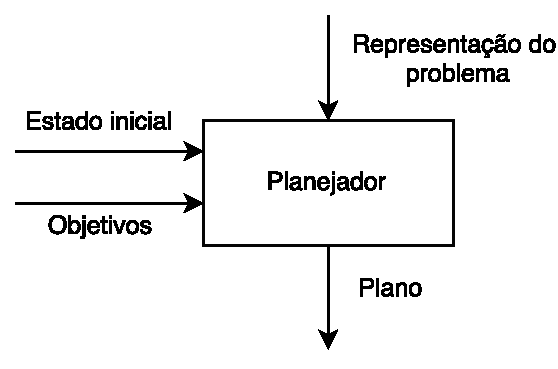
\includegraphics[width=0.4\textwidth]{fig/modelo.pdf}
	\caption{Problema de planejamento}
	\label{fig:planmodelo}
\end{figure} 


%O processo do planejamento consiste em escolher e gerenciar as ações, antecipando os resultados a fim de atingir um objetivo \cite{ghallab2004automated}.\frm{Talvez tu queira começar com busca (formalizar) e depois descer em planejamento. Aqui parece que tu cai de pára-quedas em planejamento.}

%\frm[inline]{O texto abaixo está meio confuso, tu começa falando que talvez não precise de planejamento, depois tu fala em ganhos e objetivos e mistura isto com tempo de execução do planejador. Clarifique onde tu queres chegar.}
%Para que alguns objetivos consigam ser alcançados, as ações que são tomadas não necessariamente necessitam de um planejamento, nas atividades do dia-a-dia a maioria das ações que são tomadas não são planejadas.\frm{Uh?!?! Onde tu queres chegar com isto?}
%Para fazer um planejamento é avaliado os ganhos de planejar as ações em vista do objetivo, geralmente, os planos nem sempre são os melhores possíveis, pois a busca de planos considerados perfeitos são mais demorados para construir, fazendo com que planos razoáveis ou bons sejam escolhidos ao invés dos perfeitos \cite{ghallab2004automated}. 



%Planejamento na computação é a área da Inteligencia Artificial(IA) que busca a geração de planos automaticamente de forma computacional \cite{ghallab2004automated}. 
%E para representar o processo de planejamento no computador é preciso de um modelo conceitual que é um recurso teórico usado para descrever o problema de forma geral e assim podendo aprofundar dependendo da abordagem. 
%Como planejamento é  focado na escolha de ações para acontecer mudança de estados no sistema, o modelo para descrever esse processo deve ser dinâmico, ou seja, que permita a mudança do ambiente\cite{ghallab2004automated}. 
%\frm[inline]{De novo, tudo isto acima caiu de para quedas aqui. Aqui tu situa Planejamento em IA (melhor começar com isto). Se tu começar com busca, falando de estados, ações, funções de transição, e depois falar de planejamento automático como uma formalização deste processo, o argumento vai fluir bem melhor. }

%O modelo geral utilizado para representar um plano é o \textit{state-transition systems}\frm{Um \textbf{plano}? Ou um \textbf{problema de planejamento}?}. 
%O modelo é representado por $\sum = (S, A, E, \gamma) $. Onde S representa os estados, A as ações, E os eventos que podem ocorrer no sistema, e $\gamma$ a função de transição composta por $ \gamma: S \times A \times E \rightarrow S'$. 
%A figura \ref{fig:planmodelo} ilustra uma representação desse modelo \cite{ghallab2004automated}.


%\begin{figure}[ht]
%	\centering
%	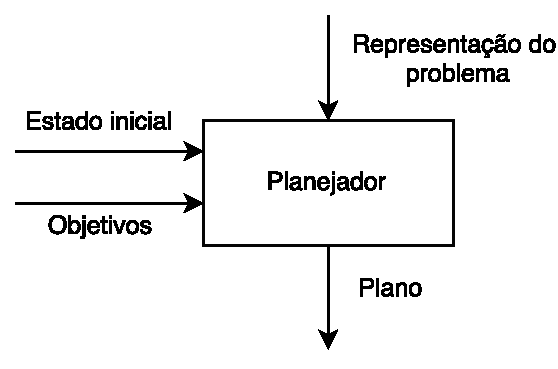
\includegraphics[width=0.4\textwidth]{fig/modelo.pdf}
%	\caption{Modelo de estado e transição}
%	\label{fig:planmodelo}
%\end{figure} 

%Um plano é gerado, quando dado um estado inicial e um objetivo, um conjunto de ações é gerado e quando executadas levam ao objetivo. \frm{Não entendi esta sentença... Evitar passivos}
%O processo usado para conseguir isso é chamado de planejamento, onde é necessário ter uma descrição do sistema($\sum$) onde os estados e as ações são definidos.\frm{$\Sigma$ é um sistema, um problema ou um plano? Te decide!! E seja preciso.}

 
%Os estados são representados por um conjunto de átomos sem função \cite{intelligence2003modern}\frm{Átomos inúteis? ou um conjunto de átomos em lógica sem símbolos de função?}, que são usados para representar alguma situação. 
%Por exemplo, o fato de uma pessoa estar em um lugar pode ser representado por \textit{at(Matheus, PUCRS)}, assim todos os estados devem seguir o padrão, podendo ter mais de uma situação, como por exemplo, representar que alguém está em um lugar e feliz ao mesmo tempo, \textit{at(Matheus,PUCRS) $\land$  happy(Matheus)}. % $\land$ fica mais legível no tex do que $\wedge$ e $\lor$ mais do que $\vee$

%As ações são descritas por um conjunto esquema de ações \cite{intelligence2003modern}\frm{Sempre que citar livro, dizer capítulo e páginas}. 
%Para toda ação é necessário uma pré condição aplicada ao estado atual, que se for satisfeita, garante o efeito ou pós condição, levando o sistema para o estado resultante. Por exemplo, caminhar de um lugar a outro: \\
%\textit{Action(walk(from, to)): \\
%Precond: at(from)  $\wedge$ path(from,to) \\
%Effect: $\neg$ at(from)  $\wedge$ at(to)}

%\frm[inline]{Exemplo disto em estados, mas talvez não precisa entrar em tanto detalhe}

\subsection{HTN} 

%\frm[inline]{Introduza o assunto mais devagar, por que HTN?}

Dentro da área de planejamento existe o planejamento \textit{Hierarchical Task Network Planning} (HTN). HTN é mais expressivo que o planejamento clássico, porque no planejamento clássico o conjunto de solução dos problemas é uma linguagem regular, ou seja, pode ser expressada por uma expressão regular, já em HTN dependendo da técnica utilizada o conjunto de solução dos problemas pode chegar a uma linguagem livre de contexto, que contém as linguagens regulares como um subconjunto, pois existem linguagens livres de contexto que não são linguagens regulares. No pior caso o resultado gerado do planejamento clássico será exponencialmente maior do que o gerado pelo planejamento HTN \cite{ghallab2004automated}.  \\

O planejamento \textit{Hierarchical Task Network} (HTN) é igual ao planejamento clássico, quando se refere a representação do problema, entretanto o diferencial vem do que é planejado e como é planejado \cite{ghallab2004automated}. \\

Em planejamento HTN as ações são tratadas em mais alto nível \cite{intelligence2003modern}. e o objetivo é achar um conjunto de tarefas que resolve determinado problema. Para isso, além da representação do problema, um conjunto de métodos é adicionado como entrada, onde este conjunto serve para decompor as tarefas em tarefas menores. O planejamento é feito decompondo tarefas não primitivas recursivamente até chegar em tarefas primitivas, que podem ser realizadas com um operador de planejamento \cite{ghallab2004automated}. Um método HTN é definido como \textit{m} = (nome(\textit{m}), tarefa(\textit{m}), subtarefas(\textit{m}), limitação(\textit{m})), onde cada elemento é definido como \cite{ghallab2004automated}: 
 
\begin{itemize}
	\item nome(\textit{m}) - Nome do método, que deve ser único, e \textit{m} é o conjunto de variaveis que será utilizado em \textit{m}. 
	\item tarefa(\textit{m}) - É uma tarefa não primitiva.
	\item (subtarefa(\textit{m}),limitação(\textit{m})) - É uma ligação de tarefa de ligação.
\end{itemize}

Uma tarefa de ligação é definida como um par w = (U,C), onde U é um conjunto de tarefas de ligação e C um conjunto de limitações. Cada limitação deve ser satisfeita em todo o plano e cada tarefa de ligação é decomposta em subtarefas até todas as tarefas se tornarem primitivas. \\

Um problema de planejamento HTN é descrito como P = ($s_{0}$, w, O, M), onde $s_{0}$ é o estado inicial, w a tarefa de ligação inicial, O é um conjunto de operadores de planejamento, e M é um conjunto de métodos. \\

Na busca pelo plano, o planejamento HTN começa planejando por um caminho, quando um caminho de resolução leva a um fim de linha é realizado um retrocesso(\textit{backtracking}) até um caminho que tenha uma possibilidade diferente de caminho do que foi tomado anteriormente.

%Os métodos de planejamento HTN são utilizados pelo fato dos problemas serem descritos como receitas, seguindo uma ordem de execução das tarefas, que pode corresponder como pessoas pensam em resolver problemas de planejamento \cite{ghallab2004automated}.  \frm{Não tenho certeza de que a relação de causalidade de (receitas $\rightarrow$ HTN) funciona da maneira que tu descreve }


%A grande diferença entre planejamento HTN e os demais tipos de planejamento é o fato de que as ações são tratadas em mais alto nível \cite{intelligence2003modern}. \frm{Todos os outros tipos de planejamento ou só planejamento clássico?}
%As ações\frm{tarefas, são decompostas, ações não!!} vão sendo decompostas até serem diretamente executadas, um bom exemplo é viajar de avião, a tarefa principal é viajar de um lugar para o outro, mas antes disso deve-se comprar a passagem e ir até o aeroporto de táxi para então conseguir realizar a viagem. 

%Em HTN as ações são chamadas de tarefas\frm{Não!!! Tarefas nem sempre são ações} e a finalidade\frm{A finalidade é alcançar um objetivo, só que isto é implícito!!} não é alcançar o objetivo, e sim realizar um conjunto de tarefas que resolvam um determinado problema. Como entrada para o sistema é necessário um conjunto de operadores e um conjunto de métodos. 
%\frm{Repetição!}
%Em HTN as ações são chamadas de tarefas, e podem ser dividas em dois tipos: Primitivas e não primitivas. 
%As tarefas primitivas são executadas diretamente através do conjunto de métodos\frm{Não!!! Reveja isto! Os métodos é que decompõe tarefas não primitivas em primitivas!!}, já as tarefas não primitivas são decompostas recursivamente em sub tarefas e assim se transformando em tarefas menores até se tornarem em tarefas primitivas, e assim podem ser executadas. 
%A Figura~\ref{fig:travelmethods} mostra um exemplo de descrição dos métodos para uma viagem de avião.\frm{Explicar a figura, note que tu não explicou métodos e ações de forma diferente.}

%\begin{figure}[ht]
%	\centering
%	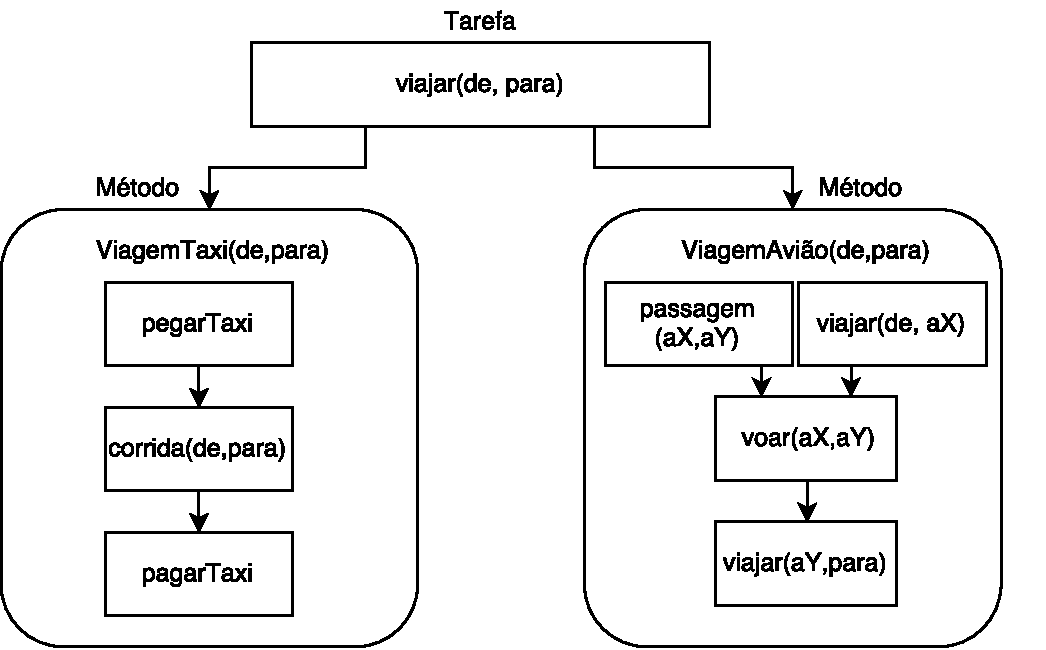
\includegraphics[width=0.8\textwidth]{fig/travelmethod.pdf}
%	\caption{Exemplo de problema de HTN}
%	\label{fig:travelmethods}
%\end{figure}  

%\frm[inline]{O planejamento HTN não executa nada (do plano) ele só planeja!!}
%O planejamento HTN executa todas as possibilidades de resolução do problema, sempre %respeitando a ordem dos métodos que conseguem ser realizados, quando um caminho de %resolução leva a um fim de linha é realizado um retrocesso(\textit{backtracking}) até um %caminho que tenha uma possibilidade de caminho diferente do que foi tomado anteriormente.

%\subsection{AHTN} 

%\textit{Adversarial hierarchical-task network} (AHTN) é um algoritmo proposto para tentar solucionar o problema do grande fator de ramificação dos jogos em tempo real \cite{ontanon2015adversarial}. O algoritmo combina técnicas de planejamento HTN e o algoritmo \textit{minimax game tree search}. 
%\frm[inline]{Incompleto! Decide se tu queres incorpora isto ao parágrafo anterior. Em tempo, acho que tu tens que falar de minimax antes, para poder fazer a ligação de HTN e minimax $\rightarrow$ AHTN}

\section{Busca adversaria}

A busca adversaria é utilizada para ambientes competitivos, como nos jogos. Como em um jogo o jogador, preferencialmente, não informa suas jogadas previamente, o ambiente se torna imprevisível, e com isso os objetivos dos jogadores entram em conflito, ambos estão em busca da vitoria. Como solução para esse problema é preciso gerar uma solução de contingencia para tentar antecipar as jogadas do adversário \cite{intelligence2003modern}. \\ 

Para explicar como resolver esse problema, primeiro é preciso considerar um jogo com dois jogadores, um é chamado de MAX e o outro de MIN. O jogador MAX começa o jogo e o jogo e então é alternado uma jogada de MIN e uma de MAX até o final do jogo. Ao final do jogo, quem vence obtém uma recompensa positiva e quem perde uma negativa. Um jogo pode ser formalizado como \cite{intelligence2003modern}:

\begin{itemize}
	\item $S_{0}$ - O estado inicial, que especifica como o jogo se configura no inicio.
	\item Jogadores(s) -  Define qual jogador tem o movimento no estado.
	\item Ações(s) - Conjunto das ações possíveis em um estado.
	\item Resultado(s, a) - Um modelo de transição, que define o resultado da ação a aplicada ao estado s.
	\item Terminal(s) - Verifica se o estado é um estado onde o jogo terminou.
	\item Utilidade(s,p) - Define qual é o valor numérico para o jogo quando atingir um estado s terminal por um jogador p. 
\end{itemize}
 
O estado inicial, as ações e os resultados definem a arvore das jogadas para o jogo. A arvore representa em cada nodo um estado do jogo e cada ligação com os níveis de baixo são os estados resultantes após a execução de cada ação possíveis para o estado. A alternância entre as jogadas de MAX e MIN até chegar as folhas da arvore que correspondem aos estados terminais. Como o ponto de vista é do MAX, o valor de cada nodo folha representa o valor de utilidade para o MAX, e os maiores valores representam bons resultados para o MAX e ruins para o MIN. Com isso o caminho resultante indica que aquela ação será a melhor ação para o estado atual. 

\msr{colocar uma figura de uma game tree?}

Este tipo de busca leva em consideração que o jogador adversário sempre realizará a jogada que mais lhe beneficiará, mas isso nem sempre acontece, seja por um descuido ou por um jogador inexperiente. Um algoritmo que utiliza deste recurso é o algoritmo \textit{minimax search}.


\section{Aprendizado} 
Para os humanos o aprendizado ocorre durante toda a vida. 
O aprendizado é o ato de adquirir novos conhecimentos, ou modificar conhecimentos já existentes ou ainda adquirir uma experiencia por repetição do ato de forma incorreta. 
Aprendizado pode variar de adquirir conhecimento de tarefas simples, como decorando um numero de telefone, até tarefas mais complicadas, como a formulação de novas teorias \cite{intelligence2003modern}. 
% Não precisa colocar quebra de parágrafo em todo o lado!

\subsection{Aprendizado de Máquina} 

A área na computação que estudo esse aprendizado de forma computacional é o aprendizado de maquina, melhor conhecida como \textit{machine learning}. A definição de aprendizado de maquina proposta por Tom Mitchell \cite{Mitchell1997ML} é a seguinte:

 \begin{quote}
 	Definição: Um programa de computador é dito que aprende de uma experiencia E com relação a alguma classe de tarefas T, e medida de performance P, se essa performance sobre as tarefas em T, medida por P, melhora com a experiencia E.
 \end{quote}

Essa definição mostra que o sistema aprimora seu conjunto de tarefas T com uma performance P através de experiencias E. Ou seja, um sistema baseado em aprendizado de maquina deve, através de experiencias, ter um ganho nas informações para solucionar os seus problemas. Para começar a resolver um problema utilizando aprendizado de maquina é preciso escolher qual experiencia será aprendida pelo sistema \cite{Mitchell1997ML}. Para isso existem algumas técnicas que tratam aprendizado de maquina com objetivos diferentes \cite{intelligence2003modern}. Alguma das técnicas são: %\frm{Olha as concordâncias!!}

%\frm[inline]{Escrever sentenças completas!}
\begin{itemize}
	\item Aprendizado supervisionado: Aprender através de algum conjunto de exemplos a realizar a classificação de algum problema. Cada problema é mapeado para uma saída. 
	\item Aprendizado não supervisionado: Aprender através das observações, algum pedrão ou regularidade, para classificar em grupos os problemas.
	\item Aprendizado por reforço: Aprender através das execuções, bem ou mal sucedidas. Aprende quais ações são melhores de ser executadas.
\end{itemize}

%\frm[inline]{Reescrever tudo isto, e organizar os pensamentos. Onde tu queres chegar com o parágrafo?}


O aprendizado por reforço também é conhecido como \textit{reinforcement learning}. O objetivo deste aprendizado é usar as recompensas obtidas nas observações para aprender uma politica do ambiente \cite{intelligence2003modern}. Para que isso aconteça, cada estado contém uma utilidade, que mostra o quão desejável é este estado, pode ser um desejo bom ou um ruim. Com essa informação é possível determinar, dado as ações disponíveis no estado, qual ação o sistema deve escolher para seguir a execução. 


%O aprendizado por reforço, também é conhecido como \textit{reinforcement learning}, \textbf{tem as técnicas }\frm{ARGH!!!} baseadas em  aprender através das execuções e a cada nova execução o conhecimento aprendido é utilizado para tentar maximizar o seu desempenho na próxima execução \cite{intelligence2003modern}. Para conseguir medir o aprendizado em cada execução, existe a abordagem que é preciso medir a quantidade do ganho por estado do sistema e assim cada estado do sistema deve ter um valor de utilidade para dizer se o estado é um estado recomendado ou não para ser alcançado, ou ainda o estado não oferece nem ganho nem perda por ser atingido. 


%\section{Jogos Real-time Strategy(RTS)} 

%Jogos eletrônicos são muito populares, não só entre os jovens, principalmente pela grande quantidade de gêneros, existem jogos de ação, aventura, esportes, estrategia, entre outros. \\
%Dentro dos jogos de estratégia há uma subseção que se chama jogos de estratégia em tempo real, neles os jogadores estão se enfrentando no mesmo momento, como o nome já diz. Em alguns desses jogos há BOTs(jogadores que simulam um jogador real) e é preciso alguma inteligencia para esses BOTs conseguirem levar graça ao jogador real, para isso é utilizado algoritmos de IA. Esse tipo de jogo, devido a sua grande quantidade de ações, possui um fator de ramificação muito grande, e cresce exponencialmente, com isso aplicar os algoritmos se torna uma tarefa não trivial.  \\